%%%%%%%%%%%%%%%%%%%%%%%%%%%%%%%%%%%%%%%%%%%%%%%%%%%%%%%%%%%%%%%%%%%%%%%
%https://www.geogebra.org/m/WRJrQRdQ?lang=de
%%%%%%%%%%%%%%%%%%%%%%%%%%%%%%%%%%%%%%%%%%%%%%%%%%%%%%%%%%%%%%%%%%%%%%%

\RequirePackage{etex}
\documentclass{beamer}
\usepackage[latin9]{inputenc}
\usepackage[ngerman]{babel}
\usepackage{amsmath}
\usepackage{listings}
\usepackage{color}
\usepackage{pictex}
\usepackage{tikz}
\usepackage{siunitx}
\usepackage{pgf}
\usepackage{mathrsfs}
\usetikzlibrary{arrows}
\usepackage{booktabs}

\title[]{Newton-Verfahren}
\author{Dominik Eisele}
\institute[WSS]{Werner-Siemens-Schule}
\date{\today}
\subject{Newton Verfahren}
\keywords{Newton, Newton-Verfahren}

\usetheme{Singapore}
\usecolortheme{rose}
\setbeamertemplate{navigation symbols}{}
\setbeamertemplate{footline}[frame number]
\beamersetuncovermixins{\opaqueness<1>{25}}{\opaqueness<2->{15}}

\definecolor{dkgreen}{rgb}{0,0.6,0}
\definecolor{gray}{rgb}{0.5,0.5,0.5}
\definecolor{mauve}{rgb}{0.58,0,0.82}
\definecolor{ffqqqq}{rgb}{255,0,0}

\lstset{language=C}
\lstset{numbers=left,
	numberstyle=\tiny,
	numbersep=5pt,
	breaklines=true,
	showstringspaces=false,
	frame=l ,
	xleftmargin=15pt,
	xrightmargin=15pt,
	basicstyle=\ttfamily\scriptsize,
	stepnumber=1,
	keywordstyle=\color{blue},		% keyword style
	commentstyle=\color{dkgreen},		% comment style
	stringstyle=\color{mauve}			% string literal style
}

%\AtBeginDocument{\addtobeamertemplate{block begin}{\setlength\abovedisplayskip{0pt}}}
%\AtBeginDocument{\addtobeamertemplate{block begin}{\setlength\abovedisplayshortskip{0pt}}}

\let\oldsqrt\sqrt
\def\sqrt{\mathpalette\DHLhksqrt}
\def\DHLhksqrt#1#2{\setbox0=\hbox{$#1\oldsqrt{#2\,}$}\dimen0=\ht0
\advance\dimen0-0.3\ht0
%0.3 ist das Ma� f�r die Hakenl�nge, relativ zum Inhalt der Wurzel
\setbox2=\hbox{\vrule height\ht0 depth -\dimen0}%
{\box0\lower0.4pt\box2}}

%\include{bild_ganze_folie.tex}

\setcounter{tocdepth}{1}

\begin{document}

\begin{frame}
	\titlepage
\end{frame}

\begin{frame}{Inhalt}
	\tableofcontents
\end{frame}


\section{Allgemeine Informationen}
\subsection{Allgemeine Informationen-dots}

\begin{frame}{Geschichte}
	\begin{itemize}
		\item wird auch Newton-Raphson-Verfahren genannt
		\item benannt nach Sir Isaac Newton (1643\,-\,1727) und Joseph Raphson (1648\,-\,1715)
		\item Raphson ver�ffentlicht vor Newton das Newton-Raphson-Verfahren speziell im Bezug auf das L�sen von Gleichungen und Wurzeln
		\item ver�ffentlicht 1736 in "`Methodus fluxionum et serierum infinitarum"'
	\end{itemize}
\end{frame}

\begin{frame}{Ziel des Newton-Verfahrens}
	\begin{itemize}
		\item Ann�herung an die Nullstellen, �ber eine Linearisierung der Funktion an geeigneten Stellen
		\item L�sung von allen nichtlinearen Gleichungen und Gleichungssystemen
		\item L�sung von Gleichungen in der Form: $f(x) = 0$
		\item kommt oft dann zum Einsatz, wenn die Gleichung nicht durch die bekannten Methoden l�sbar ist, wie z.\,B. Mitternachtsformel, quadratische
			Erg�nzung, ...
	\end{itemize}
\end{frame}

\section{Graphische Herleitung}
\subsection{Graphische Herleitung-dots}

\begin{frame}{Vorgehen bei Konstruktion}
	\begin{itemize}
		\item eine beliebige Abszisse als Startwert w�hlen, daraus den Funktionswert berechnen						\pause
		\item an die berechnete Stelle des Graphens eine Tangente anlegen									\pause
		\item den Schnittpunkt der Tangente mit der x-Achse berechnen										\pause
		\item dieser Schnittpunkt kann nun als Startwert angenommen werden									\pause
		\item die Schritte so oft wiederholen bis man die gew�nschte Genauigkeit erreicht hat
	\end{itemize}
\end{frame}

\begin{frame}{Graphische Herleitung}
	\begin{tikzpicture}[line cap=round,line join=round,>=triangle 45,x=1.0cm,y=0.4cm]
		\draw[->,color=black] (-4.2,0.) -- (4.2,0.);
		
		\foreach \x in {-4,-3,...,-1,1,2,...,4}
		\draw[shift={(\x,0)},color=black] (0pt,2pt) -- (0pt,-2pt) node[below] {\footnotesize $\x$};
		
		\draw[->,color=black] (0,-8.2) -- (0,8.2);
		
		\foreach \y in {-8,-6,...,-2,2,4,6}
		\draw[shift={(0,\y)},color=black] (2pt,0pt) -- (-2pt,0pt) node[left] {\footnotesize $\y$};
				
		\draw[color=black] (0pt,-10pt) node[right] {\footnotesize $0$};
		
		\clip(-4.2,-8.2) rectangle (4.2,8.2);
		
		\draw[color=red,smooth,samples=100,domain=-4.2:4.2] plot(\x,{0.5*(\x)^(3.0)-2.0*(\x)^(2.0)+0.5*(\x)+2.0});
		
		\begin{scriptsize}
			\draw[color=ffqqqq] (2.1,5.2) node {$g(x) = 0,5x^3 - 2x^2 + 0,5x + 2$};
		\end{scriptsize} 																	\pause
		
		\node (1) at (-1.603,0) {\textsf{X}};														\pause
		
		\draw [blue] (-1.603,0) -- (-1.603,-6);			 											\pause

		\node (2) at (-1.60298,-6) {\textsf{X}};													\pause
		
		\draw[color=green,smooth,samples=100,domain=-4.2:4.2] plot(\x,{10.76624*\x+11.25802});					\pause
		
		\node (3) at (-1.04568,0) {\textsf{X}};														\pause
		
		\draw [blue] (-1.04568,0) -- (-1.04568,-1.21842);	 											\pause
		
		\node (4) at (-1.04568,-1.21842) {\textsf{X}};												\pause
		
		\draw[color=green,smooth,samples=100,domain=-4.2:4.2] plot(\x,{6.32288*\x+5.33027});					\pause
		
		\draw[color=green,smooth,samples=100,domain=-4.2:4.2] plot(\x,{4.93807*\x+4.02045});					\pause
		
		\draw[color=green,smooth,samples=100,domain=-4.2:4.2] plot(\x,{4.75103*\x+3.86547});					\pause
		
		\draw[color=green,smooth,samples=100,domain=-4.2:4.2] plot(\x,{4.74736*\x+3.86248});					\pause
	\end{tikzpicture} 
\end{frame}

\begin{frame}{Abszissenwert}
	\begin{table}[]
		\centering
		\begin{tabular}{@{}ll@{}}
			\toprule
			Berechnungsschritt		& Abszissenwert \\ \midrule
			0                  			& -1,6029       \\
			1                  			& -1,0456       \\
			2                  			& -0,8430       \\
			3                  			& -0,8141       \\
			4                  			& -0,8136       \\
			5                  			& -0,8136       \\
			Berechneter Wert   		& -0,8136       \\ \bottomrule
		\end{tabular}
		\end{table}
\end{frame}

\section{Berechnung}
\subsection{Berechnung-dots}

\begin{frame}{Iterationsformel}
	\begin{equation*}
		\boxed{x_{n+1} = x_{n} - \frac{f(x_{n})}{f^\prime(x_{n})}}
	\end{equation*}																		\pause

	Vorgehensweise zur Berechnung von Nullstellen:													\pause
	\begin{itemize}
		\item Funktion $f(x)$ ableiten															\pause
		\item geeigneten N�herungswert als Startwert w�hlen $(x_0)$										\pause
		\item diesen f�r $x_n$ einsetzen und $x_1$ berechnen											\pause
		\item f�r $x_n$ nun $x_1$ w�hlen und $x_2$ berechnen											\pause
		\item dieses Verfahren nun so lange wiederholen bis man die gew�nschte Genauigkeit erreicht hat
	\end{itemize}
\end{frame}

\begin{frame}{Beispiel zur Iterationsformel}
	\begin{equation*}
		\boxed{x_{n+1} = x_{n} - \frac{f(x_{n})}{f^\prime(x_{n})}}
	\end{equation*}

	Vorgehensweise zur Berechnung von Nullstellen am Beispiel $f(x) = 0,5x^3 - 2x^2 + 0,5x + 2$:						\pause
	\begin{itemize}
		\item $f(x)^\prime = 1,5x^2 - 4x + 0,5$													\pause
		\item Startwert $x_0 = -1$															\pause
		\item $x_{1} = (-1) - \frac{f(-1)}{f^\prime(-1)} = (-1) - \frac{0,5 \cdot (-1)^3 - 2 \cdot (-1)^2 + 0,5 \cdot (-1) + 2}
			{1,5 \cdot (-1)^2 - 4\cdot (-1) + 0,5} \approx (-0,833)$										\pause
		\item $x_{2} = (-0,833) - \frac{0,5 \cdot (-0,833)^3 - 2 \cdot (-0,833)^2 + 0,5 \cdot (-0,833) + 2}
			{1,5 \cdot (-0,833)^2 - 4 \cdot  + 0,5} \approx (-0,814)$	\pause
		\item $x_{3} = (-0,814) - \frac{0,5 \cdot (-0,814)^3 - 2 \cdot (-0,814)^2 + 0,5 \cdot (-0,814) + 2}
			{1,5 \cdot (-0,814)^2 - 4 \cdot  + 0,5} \approx (-0,814)$
	\end{itemize}
\end{frame}

\begin{frame}{Herleitung der Iterationsformel}
	\begin{equation*}
		\boxed{x_{n+1} = x_{n} - \frac{f(x_{n})}{f^\prime(x_{n})}}
	\end{equation*}																		\pause
	
	\begin{itemize}
		\item Ziel: Nullstelle der Ableitung															\pause
		\item allgemeine Geradengleichung: $y = mx +  b$												\pause
		\item Ber�hrpunkt $P$ der Funktion mit der Tangente: $P\left( x_0 | f(x_0) \right)$							\pause
		\item Steigung an der Stelle $x_0$: $f^\prime(x_0)$
		\item Einsetzen in Geradengleichung: $f(x_0) = f^\prime(x_0) \cdot x_0  + b$ \\
			$\rightarrow b = f(x_0) - f^\prime(x_0) \cdot x_0$											\pause
		\item Einsetzen in Geradengleichung: $y = f^\prime(x_0) \cdot x  + f(x_0) - f^\prime(x_0) \cdot x_0$				\pause
		\item Nullstelle bestimmen: $0 = f^\prime(x_0) \cdot x_1  + f(x_0) - f^\prime(x_0) \cdot x_0$ \\
			$\rightarrow \boxed{x_1 =x_0 - \frac{f(x_0)}{f^\prime(x_0)}}$
	\end{itemize}
\end{frame}

\section{Fazit}
\subsection{Fazit-dots}

\begin{frame}{Vorteile des Newton Verfahrens}
	\begin{itemize}
		\item schnelle Konvergenz m�glich, da die Anzahl der signifikanten Stellen bei jeder Iteration verdoppelt wird
		\item nur ein Anfangswert n�tig
		\item in der Praxis sollte eine Hybridform aus verschiedenen Verfahren zum Einsatz kommen
		\item Nachteile k�nnen durch bessere Wahl von $x_0$ vermieden werden
	\end{itemize}
\end{frame}

\begin{frame}{Nachteile des Newton Verfahrens}
	\begin{itemize}
		\item keine Konvergenz garantiert
		\item bei Extrema oder in ihrer N�he kommt es zu Problemen, wie z.\,B. Division durch 0 bei $f^\prime(x) = 0$
	\end{itemize}
	
	\begin{figure}
		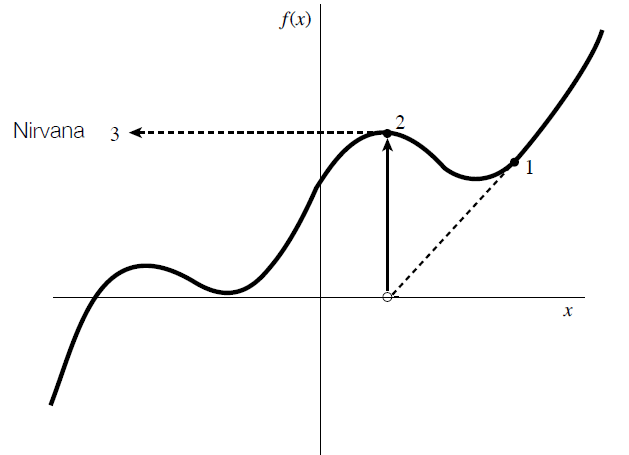
\includegraphics[width=0.5\linewidth]{Sattelstelle.png}
		\label{fig:sattelstelle}
	\end{figure}
\end{frame}

\begin{frame}{Nachteile des Newton Verfahrens}
	\begin{itemize}
		\item keine Konvergenz garantiert
		\item es kann Vorkommen dass ein nicht konvergenter Zyklus entsteht
	\end{itemize}
	
	\begin{figure}
		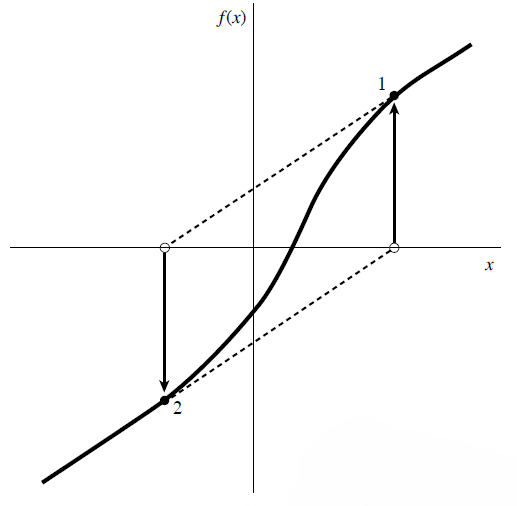
\includegraphics[width=0.5\linewidth]{Ring.png}
		\label{fig:ring}
	\end{figure}
\end{frame}

\begin{frame}{Nachteile des Newton Verfahrens}
	\begin{itemize}
		\item springen auf eine andere Nullstelle m�glich
		\item kann bei oszillierenden Funktionen vorkommen
	\end{itemize}
	
	\begin{figure}
		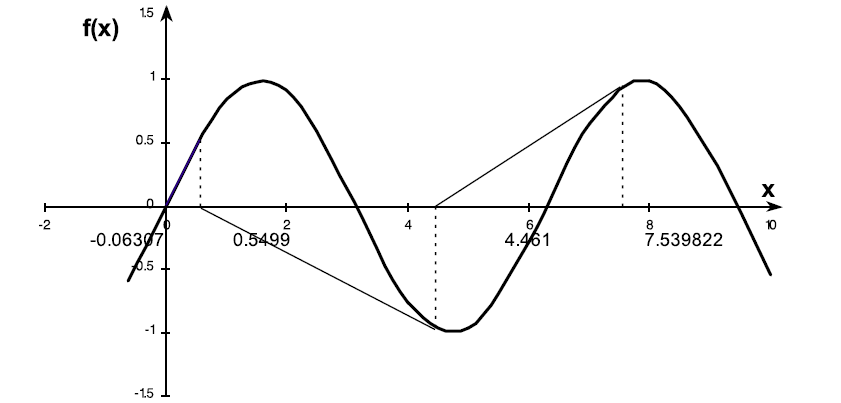
\includegraphics[width=0.7\linewidth]{hupfen.png}
		\label{fig:hupfen}
	\end{figure}
\end{frame}


\section{Anwendung}
\subsection{Anwendung-dots}

\begin{frame}{Division �ber Kehrwertbildung}
	\begin{figure}
		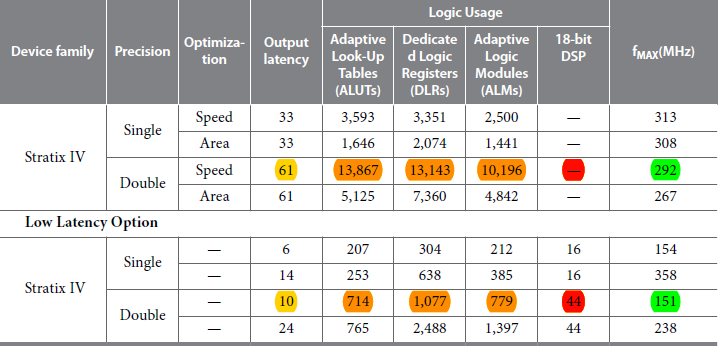
\includegraphics[width=0.8\linewidth]{Tabelle.png}
		\label{fig:Tabelle}
	\end{figure}
	\begin{itemize}
		\item beim dividieren mit Multiplizierern(rot) werden deutlich weniger Takte(gelb) ben�tigt
		\item beim dividieren mit Multiplizierern(rot) werden deutlich weniger Logikgatter(orange) ben�tigt
		\item beim dividieren ohne Multiplizierern(rot) wird eine h�here Maximalfrequenz(gr�n) erreicht
	\end{itemize}
\end{frame}

\begin{frame}{Kehrwertbildung}
	Kehrwertbildung von $A$:																	\pause
	\begin{itemize}
		\item $\frac{1}{A} = x \rightarrow 0 = \frac{1}{x} - A$											\pause
		\item Nullstelle von $f(x) = \frac{1}{x} - A$ gleich $\frac{1}{A}$										\pause
		\item $f^\prime(x) = -\frac{1}{x�}$														\pause
		\item daraus ergibt sich die Iterationsfunktion:
			$\begin{array}{rl}
				F(x)	&= x- \frac{\frac{1}{x} - A}{-\frac{1}{x�}}					\\
				F(x)	&= x \cdot (2 - A \cdot x)
			\end{array}$																\pause
		\item pro Rechenschritt nur zwei Multiplikationen und eine Addition n�tig									\pause
		\item gut Verwendbar bei Schaltungen mit schnellen Addierern 
		
	\end{itemize}
\end{frame}

\begin{frame}{Beispiel zur Kehrwertbildung}
	Kehrwertbildung von $A = 3$:											\\
	Startwert: $x_0 = 0,2$												\\
	$x_n = x \cdot (2 - A \cdot x)$											\\
	\\
	$\begin{array}{rccl}
		x_0 &	&								&= 0,2				\\
		x_1 &=& 0,2 \cdot (2 - 3 \cdot 0,2) 				&= 0,3				\\
		x_2 &=& 0,28 \cdot (2 - 3 \cdot 0,28) 				&= 0,3				\\
		x_3 &=& 0,3248 \cdot (2 - 3 \cdot 0,3248)			&= 0,333				\\
		x_4 &=& 0,33311488 \cdot (2 - 3 \cdot 0,33311488)		&= 0,333\,333			\\
		x_5 &=& 0,3333331907 \cdot (2 - 3 \cdot 0,3333331907)	&= 0,333\,333\,333\,333
	\end{array}$
\end{frame}

\section{Quellen}
\subsection{Quellen-dots}
\begin{frame}{Quellen}
	\begin{itemize}
		\item An Accurate, High Speed Implementation of Division by Reciprocal Approximation, D.L. Fowler and J.E. Smith, Astronautics Corperation of Amerika
		\item Floating-Point IP Cores User Guide
		\item Practical Numerical Training UKNum Nullstellenbestimmung (roots), PD. Dr. C. Mordasini Max Planck Institute for Astronomy, Heidelberg
		\item Rechnerarithmetik Thema: Iterative Division, Quadratwurzelberechnung, Eberhard Zehendner, Friedrich-Schiller-Universit�t Jena
		\item hs-esslingen.de/fileadmin/medien/mitarbeiter/koch/\\numerische\_methoden\_skript.pdf (Abgerufen: 08.01.2017, 02:10 Uhr)
		\item de.wikipedia.org/wiki/Newton-Verfahren (Abgerufen: 08.01.2017, 02:10 Uhr)
	\end{itemize}
\end{frame}


\end{document}
